\documentclass[10pt]{article}
\usepackage{amsmath,graphicx,xcolor,tikz,amssymb,multirow}
\usepackage[final]{pdfpages}
\usepackage{hyperref}
\usepackage{empheq}
\usepackage{fancyhdr}
\usepackage{textcomp}
\usepackage{placeins}
\usepackage{url}

\newcommand{\HRule}{\rule{\linewidth}{0.5mm}}

\newcommand{\comm}[3]{
\nonumber \textcolor{red}{?} \, \textcolor{blue}{!} \, \textcolor{red}{\text{ #1}} \,\textcolor{red}{\text{#2, }} \, \textcolor{blue}{\text{AOK.}} \, & \text{\hspace{0.5in}#3}}

\newcommand{\exchange}[2]{
\begin{equation}
 \nonumber \textcolor{red}{?} \, \textcolor{blue}{!} \, \textcolor{red}{\text { #1}} \,\textcolor{red}{\text{#2, }} \, \textcolor{blue}{\text{AOK.}}
 \end{equation}
}

\newcommand{\exchangeWithData}[2]{
\begin{equation}
 \nonumber \textcolor{red}{?} \, \textcolor{blue}{!} \, \textcolor{red}{\text { #1}} \,\textcolor{red}{\text{#2, }} \, \textcolor{blue}{data1,data2,...} \, \textcolor{blue}{AOK.}
 \end{equation}
}

\pagestyle{fancy}
\lhead{{\large Stepper Motor Controller}}
\rhead{}
\chead{}
\lfoot{{\large Imperial College CCM \the\year}}
\rfoot{\large Page \thepage}
\cfoot{}
\setlength{\headheight}{14pt} 
\renewcommand{\headrulewidth}{0.4pt}
\renewcommand{\footrulewidth}{0.4pt}

\begin{document}
\begin{titlepage}
\begin{center}

% Upper part of the page. The '~' is needed because \\
% only works if a paragraph has started.
%\includegraphics[width=0.75\textwidth]{./Figures/AO_3.png}~\\[1cm]

% Title
\HRule \\[0.4cm]
{ \huge \bfseries Stepper Motor Controller \\[0.4cm] }

\textsc{\Large RevA}\\[0.5cm]
\textsc{\Large Center for Cold Matter}\\[0.5cm]

\HRule \\[1.5cm]

\centering
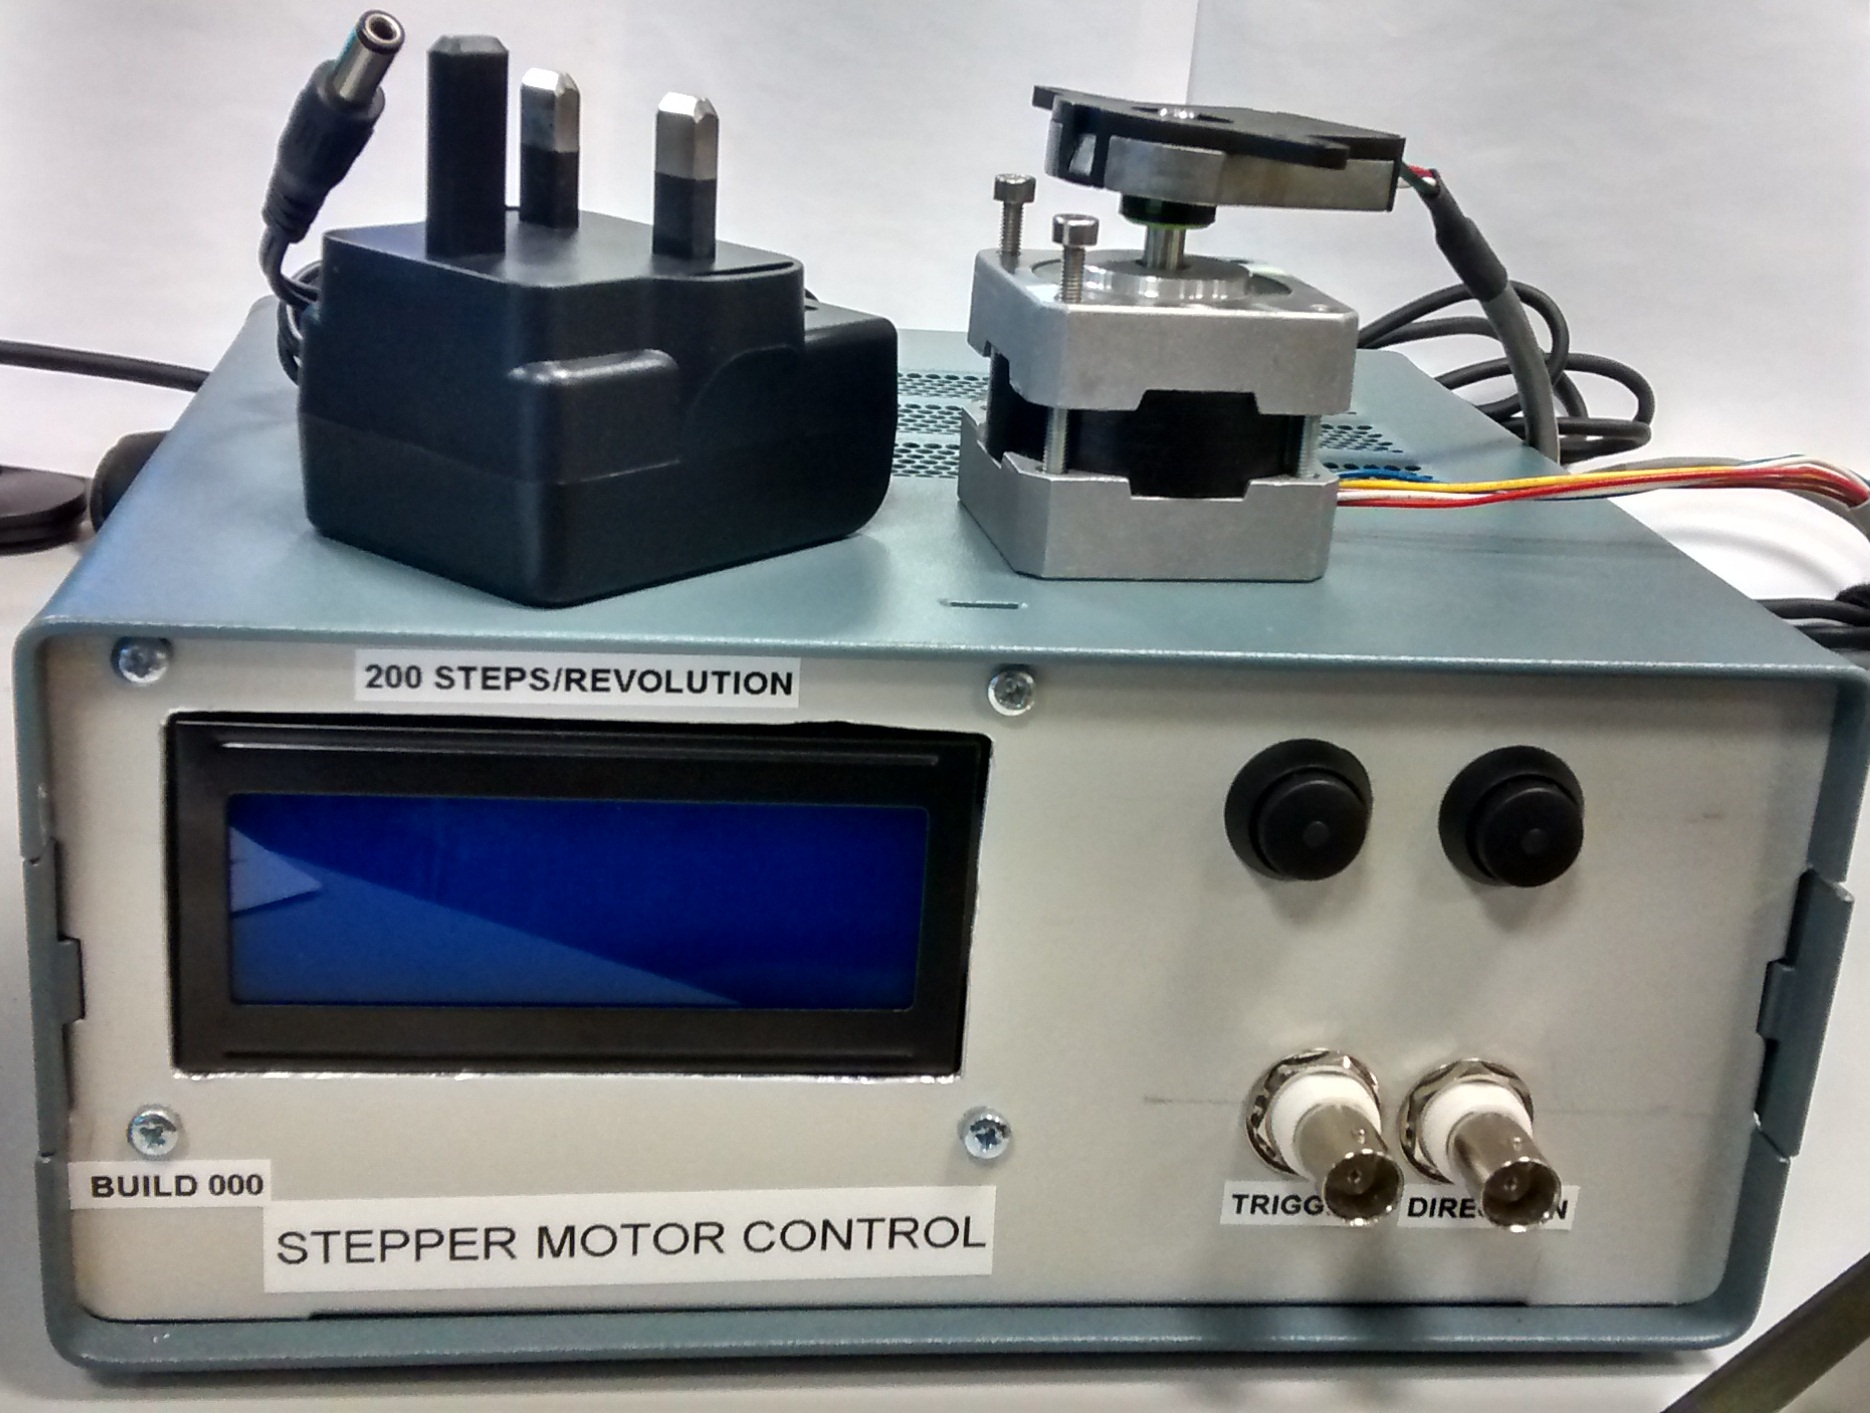
\includegraphics[width=\linewidth]{Figures/Built_Box2.jpg}

\vfill

% Bottom of the page
{\large Noah Fitch} \\
{\large \today}

\end{center}
\end{titlepage}

\newpage
\tableofcontents

\newpage
{\large{\bf Known Issues}}
\begin{enumerate}
\item{Somehow I forgot to put a pullup resistor on the $\overline{\text{MCLR}}$ line of the PIC.  In order to operate, put a 10k$\Omega$ pullup resistor to 5V.  Just under the programming connector is a convenient place (0603/0805 between that and the adjacent pin).}
\end{enumerate}

\vspace{0.5in}

{\large{\bf Minimum Requirements}}
\begin{enumerate}
\item{If using the provided GUI, you will need windows XP or newer (system has only tested on Windows 7).}
\item{If PC control/interaction with the controller is desired, you must at the very least have the FTDI COM port drivers installed.  These are included in the gui installation executable.}
\end{enumerate}

\FloatBarrier
\newpage
%%%%%%%%%%%%%%%%%%%%%%%%%%%%%%%%%%%%%%%%%%%%%%%%%%%%%%
%%%%%%%%%%%%%%%%%%%%%%%%%%%%%%%%%%%%%%%%%%%%%%%%%%%%%%%
\section{System Overview}
This circuit and associated firmware/software act as a controller for a standard unipolar (6 wire) stepper motor.  The rotary position of the motor can be controlled from a usb connection using a simple serial protocol, or with the provided gui.  In addition, a number of potentially useful predefined operation modes are available for controlling the motor.  The hardware also includes a rotation sensor, making possible both open and closed-loop operation.

All files and folders discussed in this documentation are located in the \url{CCM_0001_Unipolar_Stepper_Motor_Controller\\RevA} directory.  File and folder paths referenced herein are described \emph{relative} to this location.

%%%%%%%%%%%%%%%%%%%%%%%
\subsection{Hardware}
\label{Hardware}   
The heart of the controller is a PIC18F46K80, with a number of peripherals to facilitate motor control.  These include a DS3231M real time clock, 24AA1025 external eeprom, HCTL-2021 quadrature encoder, AMT102 rotation sensor, L297 motor driver, and power FETs for the output drive stages.  Two external bnc inputs (trigger and direction control) and two pushbuttons facilitate control of the motor by the user in various operation modes.  An LCD screen provides visual feedback of motor behaviour to the user. 

The motor used for the purpose of this documentation, and that which was used in the initial builds of the prototype circuits, is part number 191-8299 from RS components.  This is a 12V, 0.4A/phase 1.8$^\circ$/step motor.  The motor runs quite hot when supplied with the full specified voltage, for this reason the prototypes were built using a 7.5V supply instead.  The lower supply voltage sacrifices a bit of switching speed and torque but otherwise has no adverse consequences.  With these operating parameters, the fasted stepping rate is on the order of 500 Hz.  Stepping speed performance and reliability is load dependent and should be tested for the particular applications.         

%%%%%%%%%%%%%%%%%%%%%%%
\subsection{Open vs. Closed Loop Operation}
\label{Open_vs_Closed} 
Although probably not needed for most applications, the controller can be operated in closed-loop mode.  When operated this way, the current position of the motor is determined by the AMT-102 rotation sensor, rather than by how many steps the controller has instructed it to take.\footnote{The rotation sensor is set to output 800 quadrature encoded pulses per rotation.  The quadrature encoder used multiplies this by 4 so we get 16 counts for every step of the motor.}  When operated closed-loop, the controller will attempt to make this position equal to the desired position (determined by the number of triggers received in external mode, or where it thinks the motor should be in other modes).  Closed-loop operation will probably be most useful in situations where the load torque is significant, which can cause the stepping motor to ``slip'', i.e. not actually take a step even though the controlling currents toggled correctly.  If it is crucial that the motor position be accurate, it is recommended to use closed-loop mode.    

\FloatBarrier
\newpage
%%%%%%%%%%%%%%%%%%%%%%%%%%%%%%%%%%%%%%%%%%%%%%%%%%%%%%%%%
%%%%%%%%%%%%%%%%%%%%%%%%%%%%%%%%%%%%%%%%%%%%%%%%%%%%%%%%%
\section{GUI} 
\label{GUI}    

In addition to the developed firmware and hardware, there is also a provided GUI that facilitates control of the motor position and configuration of the predefined operation modes.  The GUI itself was written in Labview, which is horrible of me I know.  However, this was based on an old project and I didn't see the value in re-inventing the wheel there.    

The controller system can be installed by running
\url{gui\\Installer_Builds\\Volume\\setup.exe}.  This will carry out installation of the gui, FTDI device drivers, and Labview runtime engine.  A shortcut to the gui executable will be created on your desktop.  Updates of the gui can be carried out by simply replacing the executable itself, there is no need to rerun the entire installer.

When the gui executable is run, the first thing the back end code will do is search for a controller on the specified COM port.  The result of this test is indicated with the ``Controller Detected?'' LED.  Each time a button is depressed, and an action is taken, the ``Task Completed?'' LED will indicate the success (or lack thereof) of carrying out the desired operation.  For tasks that take a long time to execute, such as a goto, this LED will blink yellow while the task is carried out.  Explicit views of the data sent to and returned from the controller are shown in the two boxes to the left of the tab control.  Responses of AOK typically indicates the command was received and executed successfully.  ERR will indicate there was an error.  

%%%%%%%%%%%%%%%%%%%%%%%%%%%%%%%%%
\subsection{Basic Operation}
\label{Basic_Operation}
The basic operation tab of the controller gui allows for immediate control of the motor position (goto/move) as well as setting a number of operation variables.  These include uploading the current time, setting position limits, step rates, etc.    

\begin{figure}[!htb]
\centering
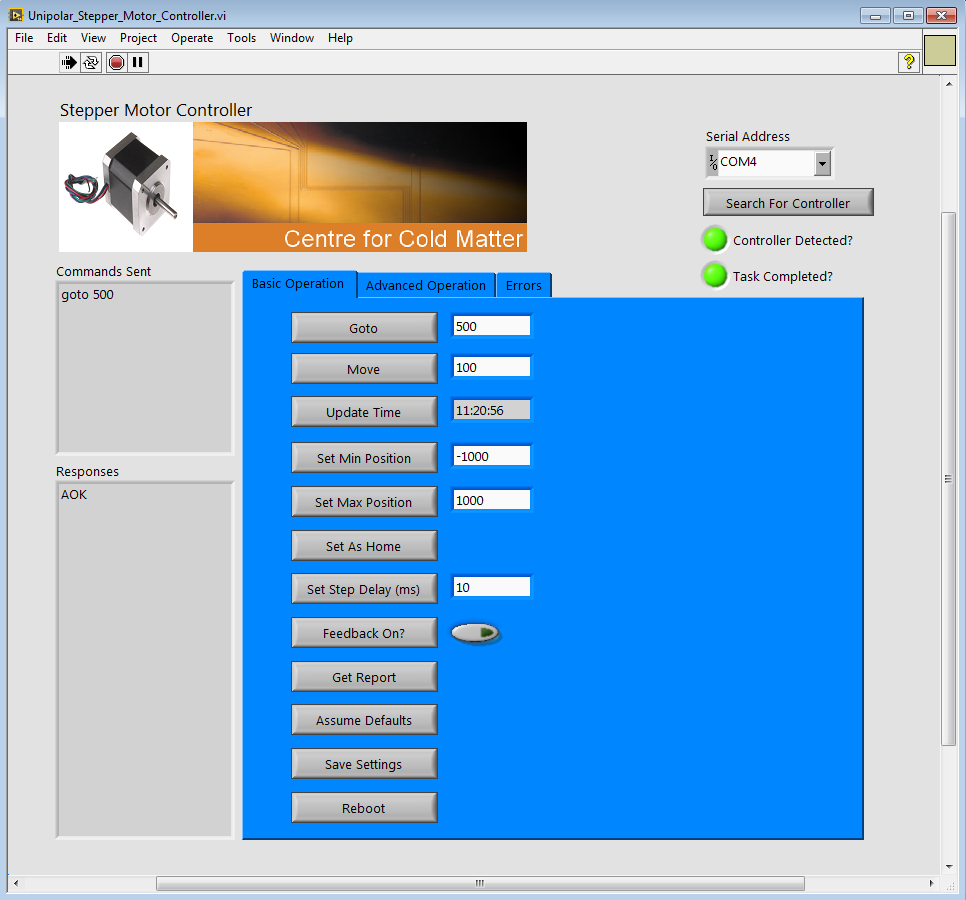
\includegraphics[width=\linewidth]{Figures/GUI_Basic_Operation.png}
\caption{Basic operation tab of the motor controller gui.}
\label{GUI_Basic_Operation}
\end{figure} 

\FloatBarrier
%%%%%%%%%%%%%%%%%%%%%%%%%%%%%%%%%
\subsection{Advanced Operation}
\label{Advanced_Operation}

The advanced operation tab (see Figure \ref{GUI_Advanced_Operation}) of the gui is used to configure the predefined operation modes native to the controller firmware.  Various configuration settings will be enabled/disabled, depending on the operation mode selected in the top dropdown menu.  The sequence of serial commands sent to the controller to configure the mode (in the Figure the triggered-goto mode has just been configured) is explained in detail in Section \ref{Configuring_Predefined_Operation_Modes}.  

\begin{figure}[!htb]
\centering
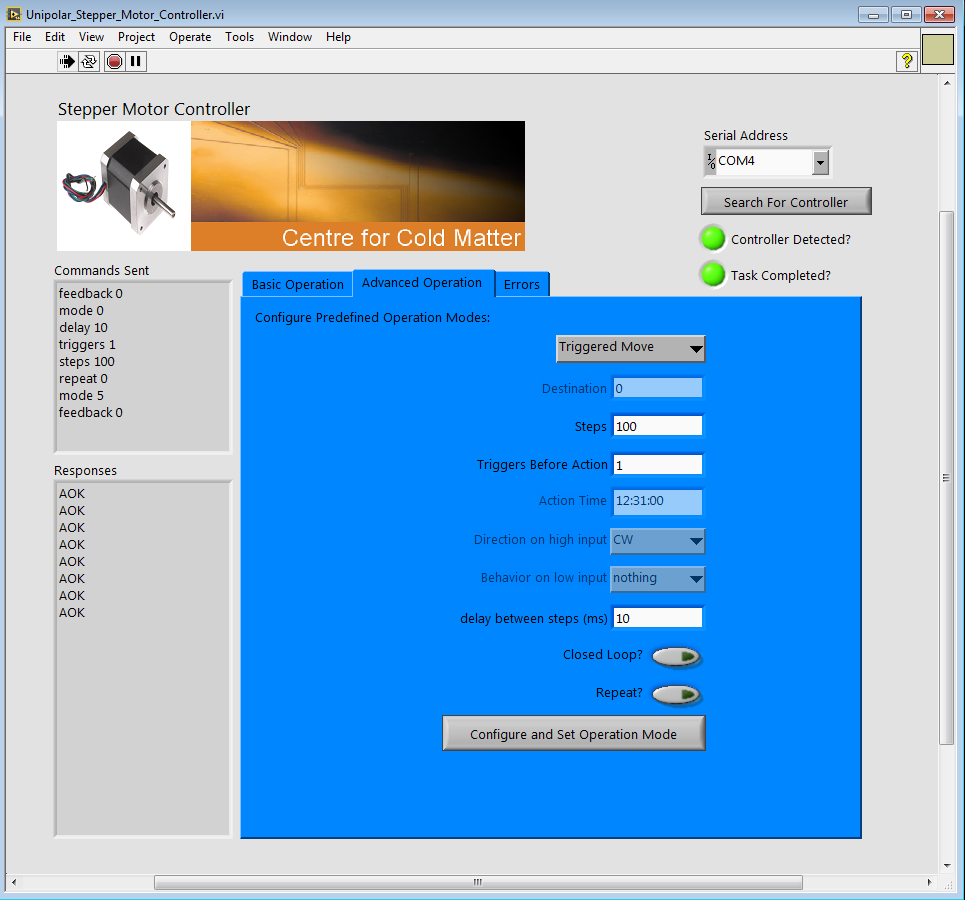
\includegraphics[width=\linewidth]{Figures/GUI_Advanced_Operation.png}
\caption{Advanced operation tab of the motor controller gui, used for configuring the predefined modes of operation.}
\label{GUI_Advanced_Operation}
\end{figure}

\subsubsection{Motor Disabled (0)}
In this mode the motor is disabled (stepping currents are turned off), allowing for free rotation.  

\subsubsection{Manual (1)}
In manual mode, the position of the motor is controlled using the two front-panel pushbuttons.  Push once to step the motor once, push and hold to continually rotate the motor.  

\subsubsection{External (2)}
In external mode, the stepping rate and direction of the motor are controlled by the two bnc inputs,  steps being taken on rising edges of the trigger input.  At the time of the rising edge of the trigger, the direction logic level determines if a positive (1) or negative (0) step is to be taken.  The direction logic input should be stable for at least $\pm$10$\mu$s around the rising trigger edge.  

\subsubsection{Triggered Goto (3)}
In triggered-goto mode, the controller is loaded with a goto destination and required number of triggers.  It then counts incoming triggers on the external bnc input (rising edges), the goto being completed when the desired number of triggers has been reached.  After completion, the controller automatically assumes manual mode.      

\subsubsection{Timed Goto (4)}
In timed-goto mode, the controller is loaded with a goto destination and action time.  The current time is monitored until a match is detected for hours/minutes/seconds, at which point the goto is completed.  After completion, the controller automatically assumes manual mode.  

\subsubsection{Triggered Move (5)}
In triggered-move mode, the controller is loaded with a step value and required number of triggers.  It then counts incoming triggers on the external bnc input (rising edges), the move being completed when the desired number of triggers has been reached.  Behaviour after the move is determined by the ``repeat'' setting.  If true, the controller resets the trigger count and prepares to repeat the move procedure once the required number of triggers has again been reached.  If false, the controller assumes the manual operation mode.  

\subsubsection{Timed Move (6)}
In timed-move mode, the controller is loaded with a step value and action time.  The current time is monitored until a match is detected for hours/minutes/seconds, at which point the move is completed.  Behaviour after the move is determined by the ``repeat'' setting.  If true, the controller resets the trigger count and prepares to repeat the move procedure once the required number of triggers has again been reached.  If false, the controller assumes the manual operation mode.

\subsubsection{State-Based Rotation (7)}
In state-rotation mode, the controller continually rotates the motor.  The rotation direction is determined by the instantaneous state of the external ``trigger'' bnc input and the ``rotate'' and ``behave'' settings, as summarized in Table \ref{State_Rotate_Table}.  When the external trigger input is high, the rotation direction is determined by the rotate setting.  When low, the motor can either do nothing (behave=0), or anti-rotate (behave=1) against the normal ``external trigger is high'' direction.  No feedback is possible during this mode.    

\begin{table}
\centering
\begin{tabular}{|c|c|c|c|}
\hline
Ext Trigger & rotate & behave & motion \\
\hline
1 & 0 & - & negative rotation \\
\hline
1 & 1 & - & positive rotation \\
\hline
0 & - & 0 & no motion \\
\hline
0 & - & 1 & anti-rotate ($\overline{\text{rotate}}$)  \\
\hline
\end{tabular}
\caption{Motor control in the ``state rotate'' operation mode is controlled by a single external input (Ext Trigger) and two internally set bits (rotate and behave).}
\label{State_Rotate_Table}
\end{table}  

\subsubsection{Triggered Shutter (8)}
In the triggered-shutter mode, the controller waits for a number of triggers (rising edges on the external trigger input) before moving the motor a specified number of steps, in effect ``opening'' a shutter.  The controller then resets the trigger count and waits for the same number of triggers before returning to the home position.  This mode repeats indefinitely.  

\subsubsection{State Shutter (9)}
In the state-shutter mode, the controller monitors the external trigger input and positions the motor in one of two places depending on the current logic state.  The direction and rotation amplitude is set by the ``steps'' variable.  This mode repeats indefinitely.  


\FloatBarrier
\newpage
%%%%%%%%%%%%%%%%%%%%%%%%%%%%%%%%%%%%%%%%%%%%%%%%%%%%%%%%%
%%%%%%%%%%%%%%%%%%%%%%%%%%%%%%%%%%%%%%%%%%%%%%%%%%%%%%%%%
\section{Serial Communication} 
\label{Serial_Communication}
In addition to the GUI, general operation and configuration of the individual predefined operation modes can be configured directly over a serial port connection.  This project uses a baud rate of 4800, 8 data bits, 1 stop bit, no port control, and no parity bit.

Each exchange between the host (PC) and the controller consists of the host giving the controller a task.  Task-dependent behaviour, including exchange of data or changing settings, can then take place.  The assignment and carrying out of each task follows a fixed protocol, as summarized in the following list. For clarity of discussion regarding communication between the host and controller, \textcolor{red}{red characters/data are sent from the host to the controller} and  \textcolor{blue}{blue characters/data are sent from the controller to the host}.   
  
\begin{enumerate}
\item{The wakeup ascii character \textcolor{red}{?} is sent to the controller to instigate communication.}
\item{When ready to receive the command, the controller returns \textcolor{blue}{!}.  If the wakeup characters was incorrect, the controller returns \textcolor{blue}{?} instead and aborts the operation.}
\item{The command, with required arguments, is sent to the controller.  If a command has arguments, the command and it's arguments are separated by a space.  The command/argument sequence terminates with a carriage return ascii character (CR, 0x13) or line feed (LF, 0x10).\footnote{Technically, \emph{any} non-alphabetic or numeric ascii character will work, other than a space.}}
\item{The controller carries out the specified task.}
\item{The controller ends the current task by sending "AOK" if the task was carried out without errors, or "ERR" if an error occurred, potentially with an error message, terminated by a line feed (LF, 0x10).}
\end{enumerate}

An example of adjusting settings on the controller from a serial port terminal (TeraTerm in this case) is shown in Figure \ref{Serial_Example}.  The terminal is setup to echo host keyboard entries to the screen.  As shown, each command begins with the exchange of ``?'' (sent by the host), with ``!'' returned from the controller.    

\begin{figure}[!htb]
\centering
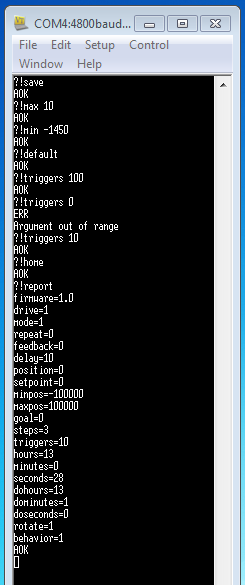
\includegraphics[width=0.5\linewidth]{Figures/Terminal.png}
\caption{Example interaction with the controller over USB using individual commands sent from teraterm.}
\label{Serial_Example}
\end{figure} 

\FloatBarrier
%%%%%%%%%%%%%%%%%%%%%%%%%%%%%%%%%%%%%%%%%%
\subsection{Available Commands}

Available commands sent to the controller and brief description of the associated task are summarized in Table \ref{commands}.  The ``goto'' and ``move'' commands are used for immediate motor operation.  Some of the other commands are only used in certain operation modes.        

\begin{table}[!hb]
\centering
\begin{tabular}{|c|c|c|}
\hline
Command & 
Description & 
used in modes 
\\
\hline
\hyperref[report]{report} & 
report current settings &
-
\\ \hline
\hyperref[default]{default} & 
assume default values &
-
\\ \hline
\hyperref[save]{save} & 
save settings &
-
\\ \hline
\hyperref[home]{home} & 
set position as home &
-
\\ \hline
\hyperref[reboot]{reboot} & 
reboot the controller &
-
%\\ \hline
%\hyperref[update]{update} & 
%update firmware &
%-
\\ \hline
\hyperref[move]{move} & 
move the motor N steps &
-
\\ \hline
\hyperref[goto]{goto} & 
goto position &
-
\\ \hline
\hyperref[max]{max} & 
set maximum position &
all
\\ \hline
\hyperref[min]{min} & 
set minimum position &
all
\\ \hline
\hyperref[delay]{delay} & 
set delay between steps &
all
\\ \hline
\hyperref[feedback]{feedback} & 
set feedback on/off &
all
\\ \hline
\hyperref[mode]{mode} & 
set operation mode &
-
\\ \hline
\hyperref[steps]{steps} & 
set number of steps &
5,6,8,9
\\ \hline
\hyperref[triggers]{triggers} & 
set trigger events before action&
3,5,8
\\ \hline
\hyperref[goal]{goal} & 
set destination &
3,4
\\ \hline
\hyperref[hours]{hours} & 
set current time (hours) &
4,6
\\ \hline
\hyperref[minutes]{minutes} & 
set current time (minutes) &
4,6
\\ \hline
\hyperref[seconds]{seconds} & 
set current time (seconds) &
4,6
\\ \hline
\hyperref[dohours]{dohours} & 
set action time (hours) &
4,6
\\ \hline
\hyperref[dominutes]{dominutes} & 
set action time (minutes) &
4,6
\\ \hline
\hyperref[doseconds]{doseconds} & 
set action time (seconds) &
4,6
\\ \hline
\hyperref[repeat]{repeat} & 
set loop behaviour condition &
5,6
\\ \hline
\hyperref[rotate]{rotate} & 
set rotation direction for logic high input &
7
\\ \hline
\hyperref[behave]{behave} & 
set state-rotate behaviour for logic low input &
7
\\ \hline
\end{tabular}
\caption{Available commands to send to the controller from the host.}
\label{commands}
\end{table} 

Examples of the usage of each command in Table \ref{commands} appears below.  Some commands require arguments, while others do not.
In each example, commas (,) indicate carriage returns and periods (.) indicate line feeds.  

%%%%%%%%%%%%%%%%%%%%%%%%%
\subsubsection{report}
\label{report}
Instructs the controller to return a list of the current settings, each setting is of the format ``setting$=$value'', with a carriage return between each list entry. 

\exchangeWithData{report}{} 

%%%%%%%%%%%%%%%%%%%%%%%%%
\subsubsection{default}
\label{default}
Instructs the controller to restore default values. 

\exchange{default}{}

%%%%%%%%%%%%%%%%%%%%%%%%%
\subsubsection{save}
\label{save}
Instructs the controller to save the current settings.  These will be restored if the controller is reset.

\exchange{save}{}

%%%%%%%%%%%%%%%%%%%%%%%%%
\subsubsection{home}
\label{home} 
Instructs the controller to set the current position as home (0).

\exchange{home}{}
    
%%%%%%%%%%%%%%%%%%%%%%%%%
\subsubsection{reboot}
\label{reboot}
Carries out a restart of the controller equivalent to that during a hard power supply cycle.  The communication flow looks like:    

\exchange{reboot}{}

%%%%%%%%%%%%%%%%%%%%%%%%%
%\subsubsection{update}
%\label{update}
%Invokes the bootloader on the controller, in order to carry out a firmware update.  %This should be used in conjunction with the ds30 bootloader utilities, available in %the \url{bootloader\\ds30} directory.  The communication flow follows:    

%\exchange{update}{}

%%%%%%%%%%%%%%%%%%%%%%%%%
\subsubsection{move}
\label{move}
Moves the motor a specified number of steps. The number of steps must be between -2000000 and 2000000.         

\exchange{move}{-100}

%%%%%%%%%%%%%%%%%%%%%%%%%
\subsubsection{goto}
\label{goto}
Moves the motor to a specified position. The destination must be between -1000000 and 1000000.         

\exchange{goto}{1000}

%%%%%%%%%%%%%%%%%%%%%%%%%
\subsubsection{max}
\label{max}
Set the maximum allowed motor position, -1000000 to 1000000.         

\exchange{max}{10000}

%%%%%%%%%%%%%%%%%%%%%%%%%
\subsubsection{min}
\label{min}
Set the minimum allowed motor position, -1000000 to 1000000.         

\exchange{min}{-10000}

%%%%%%%%%%%%%%%%%%%%%%%%%
\subsubsection{delay}
\label{delay}
Set the approximate delay time between steps (for moves, gotos, etc.), 10-65535 (ms).         This is not a guaranteed timescale, the user should test for themselves if precise timing is required. 

\exchange{delay}{10}

%%%%%%%%%%%%%%%%%%%%%%%%%
\subsubsection{feedback}
\label{feedback}
Instructs the controller to turn the feedback off (0) or on (1). 

\exchange{feedback}{0}

%%%%%%%%%%%%%%%%%%%%%%%%%
\subsubsection{mode}
\label{mode}
Set the operation mode, as summarized in Table \ref{Operation_Modes_Table}.  The destination mode should be fully configured before transferring.   

\exchange{mode}{1}

\begin{table}[!htb]
\centering
\begin{tabular}{|c|c|c|}
\hline
Mode & Behaviour \\ \hline
0 & motor disabled \\ \hline
1 & manual \\ \hline
2 & external \\ \hline
3 & triggered goto \\ \hline
4 & timed goto \\\hline
5 & triggered move \\ \hline
6 & timed move \\ \hline
7 & state-based rotation \\ \hline
8 & triggered shutter \\ \hline
9 & state-based shutter \\ \hline
\end{tabular}
\caption{Pre-defined operation modes.}
\label{Operation_Modes_Table}
\end{table}

%%%%%%%%%%%%%%%%%%%%%%%%%
\subsubsection{steps}
\label{steps}
Set the number of steps, -2000000 to 2000000.  Used to configure various predefined operation modes (shutter and move modes).

\exchange{steps}{87}

%%%%%%%%%%%%%%%%%%%%%%%%%
\subsubsection{triggers}
\label{triggers}
Set the number of triggers (rising edges on external trigger input) before action is to be taken.  The allowed range is 1-65535.  This parameter is used for various predefined operation modes.

\exchange{triggers}{10}

%%%%%%%%%%%%%%%%%%%%%%%%%
\subsubsection{goal}
\label{goal}
Set the destination for goto-style predefined operation modes.

\exchange{goal}{-145}

%%%%%%%%%%%%%%%%%%%%%%%%%
\subsubsection{hours}
\label{hours}
Set the current time (hours, 0-23).  Used for time-dependent operation modes.

\exchange{hours}{12}

%%%%%%%%%%%%%%%%%%%%%%%%%
\subsubsection{minutes}
\label{minutes}
Set the current time (minutes, 0-59). Used for time-dependent operation modes.

\exchange{minutes}{30}

%%%%%%%%%%%%%%%%%%%%%%%%%
\subsubsection{seconds}
\label{seconds}
Set the current time (seconds, 0-59). Used for time-dependent operation modes.

\exchange{seconds}{30}

%%%%%%%%%%%%%%%%%%%%%%%%%
\subsubsection{dohours}
\label{dohours}
Set the action time (hours, 0-23).  Used for time-dependent operation modes.

\exchange{dohours}{12}

%%%%%%%%%%%%%%%%%%%%%%%%%
\subsubsection{dominutes}
\label{dominutes}
Set the action time (minutes, 0-59). Used for time-dependent operation modes.

\exchange{dominutes}{30}

%%%%%%%%%%%%%%%%%%%%%%%%%
\subsubsection{doseconds}
\label{doseconds}
Set the action time (seconds, 0-59). Used for time-dependent operation modes.

\exchange{doseconds}{30}

%%%%%%%%%%%%%%%%%%%%%%%%%
\subsubsection{repeat}
\label{repeat}
Set the repetition behaviour for various operation modes, such as a triggered move. If turned off (0), after the move is completed, the operation mode will be set to manual.  If turned on (1), the mode will remain unchanged and the desired operation will repeat again once the necessary conditions are met (triggers received or time-of-day match etc.). 

\exchange{repeat}{1}

%%%%%%%%%%%%%%%%%%%%%%%%%
\subsubsection{rotate}
\label{rotate}
Used for rotate mode.  Instructs the motor which way to rotate for a logic high on the external trigger input.   

\exchange{rotate}{1}

%%%%%%%%%%%%%%%%%%%%%%%%%
\subsubsection{behave}
\label{behave}
Set the rotation behaviour in the state-rotate mode when the external trigger bnc input is logic low.  If 0, the motor does nothing for a logic-low input.  If 1, the motor anti-rotates in the direction opposite of that determined by the ``rotate'' setting. 

\exchange{behave}{0} 


%%%%%%%%%%%%%%%%%%%%%%%%%%%%%%%%%%%%%%%%%%
\subsection{Configuring Predefined Operation Modes via USB}
\label{Configuring_Predefined_Operation_Modes}
Configuring the predefined operation modes over USB, rather than the GUI, consists of completing a sequence of exchanges with the controller.  It is recommended that when configuring a mode, the first few commands disable the motor and turn the feedback off.  This will ensure that the subsequent commands, used to configure the mode, can be carried out without the motor undergoing uncontrolled motion.  If removing the motor drive during configuration is a concern, the manual mode of operation can be assumed instead.  Examples of configuring each mode using the serial port follow.  Some settings will not need to be configured separately for each mode as shown, depending on the values before configuration.    

\subsubsection{Configuring ``Off'' Mode}
\begin{align}
\comm{feedback}{0}{disable feedback} \\
\comm{mode}{0}{disable motor} \\
\nonumber
\end{align}

\subsubsection{Configuring ``Manual'' Mode}
\begin{align}
\comm{feedback}{0}{disable feedback} \\
\comm{mode}{0}{disable motor} \\
\comm{delay}{x}{set delay between steps} \\
\comm{mode}{1}{set mode to manual} \\
\comm{feedback}{1}{turn feedback on (if desired)} \\
\nonumber
\end{align}

\subsubsection{Configuring ``External'' Mode}
\begin{align}
\comm{feedback}{0}{disable feedback} \\
\comm{mode}{0}{disable motor} \\
\comm{mode}{2}{set mode to external} \\
\comm{feedback}{1}{turn feedback on (if desired)} \\
\nonumber
\end{align}

\subsubsection{Configuring ``Triggered Goto'' Mode}
\begin{align}
\comm{feedback}{0}{disable feedback} \\
\comm{mode}{0}{disable motor} \\
\comm{delay}{a}{set delay between steps, ms (a)} \\
\comm{triggers}{b}{set number of triggers before goto completed (b)} \\
\comm{goal}{c}{set destination position (c)} \\
\comm{mode}{3}{set mode to triggered goto} \\
\comm{feedback}{1}{turn feedback on (if desired)} \\
\nonumber
\end{align}

\subsubsection{Configuring ``Timed Goto'' Mode}
\begin{align}
\comm{feedback}{0}{disable feedback} \\
\comm{mode}{0}{disable motor} \\
\comm{delay}{a}{set delay between steps, ms (a)} \\
\comm{hours}{b}{set current time, hours (b)} \\
\comm{minutes}{c}{set current time, minutes (c)} \\
\comm{seconds}{d}{set current time, seconds (d)} \\
\comm{dohours}{e}{set action time, hours (e)} \\
\comm{dominutes}{f}{set action time, minutes (f)} \\
\comm{doseconds}{g}{set action time, seconds (g)} \\
\comm{goal}{h}{set destination position (h)} \\
\comm{mode}{4}{set mode to timed goto} \\
\comm{feedback}{1}{turn feedback on (if desired)} \\
\nonumber
\end{align}

\subsubsection{Configuring ``Triggered Move'' Mode}
\begin{align}
\comm{feedback}{0}{disable feedback} \\
\comm{mode}{0}{disable motor} \\
\comm{delay}{a}{set delay between steps, ms (a)} \\
\comm{triggers}{b}{set number of triggers before goto completed (b)} \\
\comm{steps}{c}{set number of steps to take (c)} \\
\comm{mode}{5}{set mode to triggered move} \\
\comm{feedback}{1}{turn feedback on (if desired)} \\
\nonumber
\end{align}

\subsubsection{Configuring ``Timed Move'' Mode}
\begin{align}
\comm{feedback}{0}{disable feedback} \\
\comm{mode}{0}{disable motor} \\
\comm{delay}{a}{set delay between steps, ms (a)} \\
\comm{hours}{b}{set current time, hours (b)} \\
\comm{minutes}{c}{set current time, minutes (c)} \\
\comm{seconds}{d}{set current time, seconds (d)} \\
\comm{dohours}{e}{set action time, hours (e)} \\
\comm{dominutes}{f}{set action time, minutes (f)} \\
\comm{doseconds}{g}{set action time, seconds (g)} \\
\comm{steps}{h}{set number of steps to take (h)} \\
\comm{mode}{6}{set mode to timed move} \\
\comm{feedback}{1}{turn feedback on (if desired)} \\
\nonumber
\end{align}

\subsubsection{Configuring ``State Rotate'' Mode}
\begin{align}
\comm{feedback}{0}{disable feedback} \\
\comm{mode}{0}{disable motor} \\
\comm{delay}{a}{set delay between steps, ms (a)} \\
\comm{rotate}{b}{set direction to rotate on high input (b)} \\
\comm{behave}{c}{set behaviour on low input (c)} \\
\comm{mode}{7}{set mode to state rotate} \\
\nonumber
\end{align}

\subsubsection{Configuring ``Triggered Shutter'' Mode}
\begin{align}
\comm{feedback}{0}{disable feedback} \\
\comm{mode}{0}{disable motor} \\
\comm{delay}{a}{set delay between steps, ms (a)} \\
\comm{triggers}{b}{set trigger number for opening/closing (b)} \\
\comm{steps}{c}{set number of steps to take (c)} \\
\comm{mode}{8}{set mode to triggered shutter} \\
\comm{feedback}{1}{turn feedback on (if desired)} \\
\nonumber
\end{align}

\subsubsection{Configuring ``State Shutter'' Mode}
\begin{align}
\comm{feedback}{0}{disable feedback} \\
\comm{mode}{0}{disable motor} \\
\comm{delay}{a}{set delay between steps, ms (a)} \\
\comm{steps}{b}{set number of steps to take (b)} \\
\comm{mode}{9}{set mode to state shutter} \\
\comm{feedback}{1}{turn feedback on (if desired)} \\
\nonumber
\end{align}

\newpage
\FloatBarrier
%%%%%%%%%%%%%%%%%%%%%%%%%%%%%%%%%%%%%%%%%%%%%%%   
%%%%%%%%%%%%%%%%%%%%%%%%%%%%%%%%%%%%%%%%%%%%%%%
\section{Prototype Builds}
\label{Prototype_Builds} 



\newpage
\FloatBarrier
%%%%%%%%%%%%%%%%%%%%%%%%%%%%%%%%%%%%%%%%%%%%%%%   
%%%%%%%%%%%%%%%%%%%%%%%%%%%%%%%%%%%%%%%%%%%%%%%
\section{Circuit Schematics}
\label{Circuit_Schematics}    

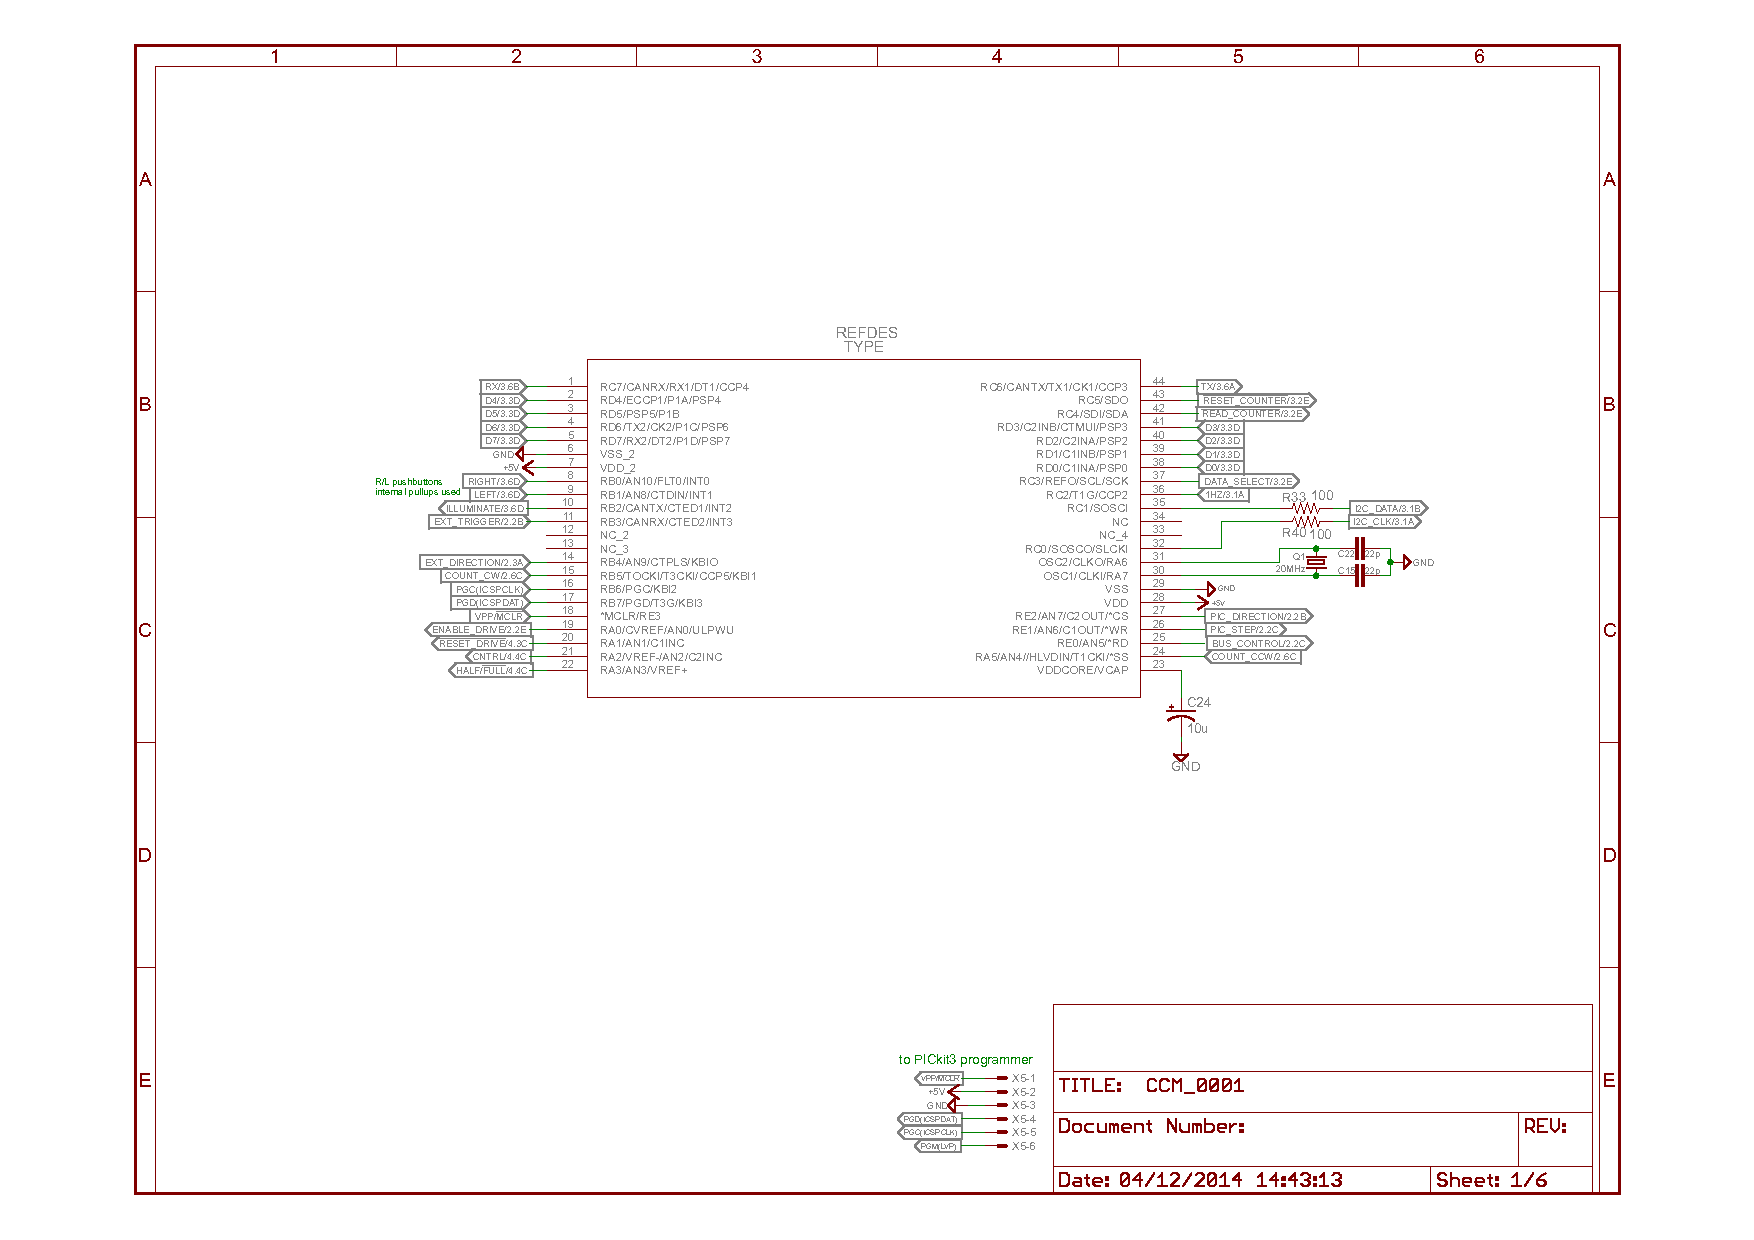
\includepdf			
[pages=-,angle=90,pagecommand={},width=6.5in,height=9in]
{Figures/CCM_0001.pdf}

\end{document} 